\documentclass[aspectratio=169]{beamer}

\usepackage{animate}
\usepackage[utf8]{inputenx} % For æ, ø, å
\usepackage{csquotes}       % Quotation marks
\usepackage{microtype}      % Improved typography
\usepackage{amssymb}        % Mathematical symbols
\usepackage{mathtools}      % Mathematical symbols
\usepackage[absolute, overlay]{textpos} % Arbitrary placement
\setlength{\TPHorizModule}{\paperwidth} % Textpos units
\setlength{\TPVertModule}{\paperheight} % Textpos units
\usepackage{tikz}
\usetikzlibrary{overlay-beamer-styles}  % Overlay effects for TikZ

\AtBeginSection{\frame{\sectionpage}}
\AtBeginSubsection{\frame{\subsectionpage}}

\usepackage{hyperref}
\usepackage{svg}
%\usefonttheme{serif}

\usepackage{xfrac}
\usepackage{color, soul, xcolor} % Colored text and highlighting, respectively
\makeatletter
\let\HL\hl
\renewcommand\hl{%
  \let\set@color\beamerorig@set@color
  \let\reset@color\beamerorig@reset@color
  \HL}
\makeatother
\usepackage{tikz-cd} % For commutative diagrams
\usepackage{tikz-3dplot}
\usetikzlibrary{angles}
\RequirePackage{pgfplots}
\usepackage{mathtools}
\usepackage{answers}
\usepackage{setspace}
\usepackage{graphicx}
\usepackage{enumerate}
\usepackage{multicol}
\usepackage{mathrsfs}
\usepackage{amsmath,amsthm,amssymb}
\usepackage{marvosym,wasysym} %fucking smileys
\usepackage{float}
\usepackage{morefloats}
\usepackage{pgf,tikz}
\pgfplotsset{compat=1.15}
\usepackage{mathrsfs}
\usetikzlibrary{arrows}
\usepackage{subcaption}
\usepackage[most]{tcolorbox}
\tcbuselibrary{theorems}
\usepackage{fancyvrb}
\usepackage{longtable,booktabs}
\usepackage{stackrel}
\usepackage{animate}
\usepackage[percent]{overpic}
\definecolor{lighter_csu_green}{RGB}{60,133,77}
\newcommand\boldgreen[1]{\textcolor{lighter_csu_green}{\emph{\textbf{#1}}}}
\usepackage{MnSymbol}
%border matrix
\makeatletter
\newif\if@borderstar
\def\bordermatrix{\@ifnextchar*{%
\@borderstartrue\@bordermatrix@i}{\@borderstarfalse\@bordermatrix@i*}%
}
\def\@bordermatrix@i*{\@ifnextchar[{\@bordermatrix@ii}{\@bordermatrix@ii[()]}}
\def\@bordermatrix@ii[#1]#2{%
\begingroup
\m@th\@tempdima8.75\p@\setbox\z@\vbox{%
\def\cr{\crcr\noalign{\kern 2\p@\global\let\cr\endline }}%
\ialign {$##$\hfil\kern 2\p@\kern\@tempdima & \thinspace %
\hfil $##$\hfil && \quad\hfil $##$\hfil\crcr\omit\strut %
\hfil\crcr\noalign{\kern -\baselineskip}#2\crcr\omit %
\strut\cr}}%
\setbox\tw@\vbox{\unvcopy\z@\global\setbox\@ne\lastbox}%
\setbox\tw@\hbox{\unhbox\@ne\unskip\global\setbox\@ne\lastbox}%
\setbox\tw@\hbox{%
$\kern\wd\@ne\kern -\@tempdima\left\@firstoftwo#1%
\if@borderstar\kern2pt\else\kern -\wd\@ne\fi%
\global\setbox\@ne\vbox{\box\@ne\if@borderstar\else\kern 2\p@\fi}%
\vcenter{\if@borderstar\else\kern -\ht\@ne\fi%
\unvbox\z@\kern-\if@borderstar2\fi\baselineskip}%
\if@borderstar\kern-2\@tempdima\kern2\p@\else\,\fi\right\@secondoftwo#1 $%
}\null \;\vbox{\kern\ht\@ne\box\tw@}%
\endgroup
}
\makeatother

\usetheme{UiB}

%For easier reading
\setbeamersize{text margin left=40pt,text margin right=40pt}
\renewcommand{\baselinestretch}{1.3}


%% FONT STUFF
\usepackage{amsmath}
\usepackage{amsfonts}
\usefonttheme[onlymath]{serif}

%Commands
\newcommand{\R}{\mathbb{R}}
\newcommand{\C}{\mathbb{C}}
\newcommand{\state}{\boldsymbol{x}}
\newcommand{\observation}{\boldsymbol{z}}
\newcommand{\obsop}{\boldsymbol{H}}
\newcommand{\modelerror}{\boldsymbol{\sigma}}
\newcommand{\modelcovariance}{\boldsymbol{\Sigma}}
\newcommand{\observationerror}{\boldsymbol{r}}
\newcommand{\observationcovariance}{\boldsymbol{R}}
\newcommand{\modelf}{\boldsymbol{F}}
\newcommand{\weights}{\boldsymbol{w}}
\newcommand{\prob}{\operatorname{p}}
\newcommand{\snapshot}{\boldsymbol{X}}


\author{Colin Roberts}
\setbeamercolor{title}{fg=white} 
\title{Model and Data Reduction Techniques for Data Assimilation}
\setbeamercolor{subtitle}{fg=white} 
%\subtitle{}



\begin{document}

%%%%%%%%%%%%%%%%%%%%%%%%%%%%%%%%%%%%%%%%%%%%%%%%%%%%%%%%%%%%%%%%%%%%%%%%%%%%%%%%%%%%%%%%%%%%%%%%%%%%%%%%%%%%

\begin{frame}{Introduction}
\pause
\vfill
\textbf{\underline{Question:}} What is data assimilation?
\begin{itemize}
    \pause
    \item ``\boldgreen{Data assimilation} is the technique whereby observational \boldgreen{data} are combined with output from a numerical \boldgreen{model} to produce an optimal estimate of the evolving state of the system.'' \quad -Alan O'Neill
\end{itemize}
\vfill
\end{frame}

%%%%%%%%%%%%%%%%%%%%%%%%%%%%%%%%%%%%%%%%%%%%%%%%%%%%%%%%%%%%%%%%%%%%%%%%%%%%%%%%%%%%%%%%%%%%%%%%%%%%%%%%%%%%

\begin{frame}{Motivation}
    \vfill
    \begin{columns}
    \begin{column}{.49\textwidth}
    \begin{itemize}
        \pause
        \item Say we are given this satellite data taken over various times.
        \item We want to fill in the missing data given these measurements and a model.
    \end{itemize}
    \end{column}

 \begin{column}{.49\textwidth}
        \begin{figure}[h]
            \centering
            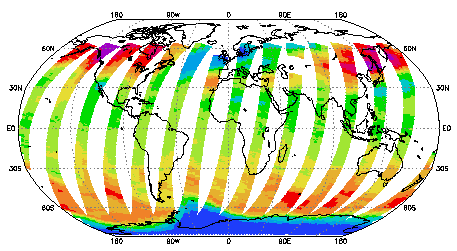
\includegraphics[width=40mm]{figures/gome_data.png}
            \caption{GOME, TM3-DAM data.}
        \end{figure}
 \end{column}
\end{columns}
\vfill
\end{frame}

\begin{frame}{Motivation}
    \vfill
    \begin{columns}
    \begin{column}{.49\textwidth}
    \begin{itemize}
        \item Say we are given this satellite data taken over various times.
        \item \hl{We want to fill in the missing data given these measurements and a model.}
    \end{itemize}
    \end{column}

 \begin{column}{.49\textwidth}
        \begin{figure}[h]
            \centering
            \vspace*{3.5mm}
            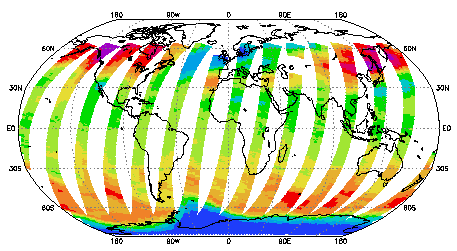
\includegraphics[width=40mm]{figures/gome_data.png}
            \caption{GOME, TM3-DAM data.}
        \end{figure}
 \end{column}
\end{columns}
\vfill
\end{frame}

%%%%%%%%%%%%%%%%%%%%%%%%%%%%%%%%%%%%%%%%%%%%%%%%%%%%%%%%%%%%%%%%%%%%%%%%%%%%%%%%%%%%%%%%%%%%%%%%%%%%%%%%%%%%

\begin{frame}{Motivation}
\vfill
    \begin{columns}
    \begin{column}{.49\textwidth}
    \begin{itemize}
        \item Not just an interpolation tool!
        \item Data assimilation is used to improve forecasts as well.
    \end{itemize}
    \end{column}

 \begin{column}{.49\textwidth}
        \begin{figure}[h]
            \centering
            \vspace*{3.5mm}
            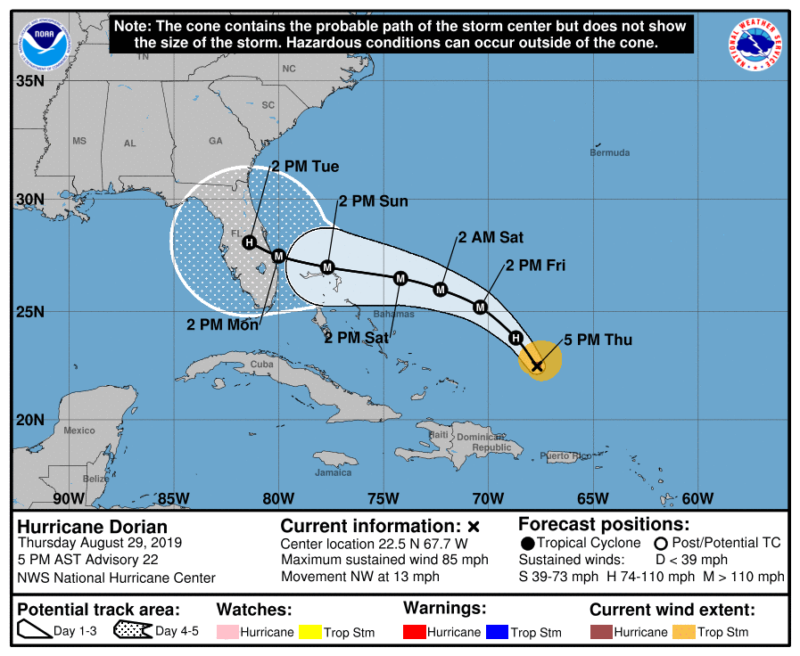
\includegraphics[width=40mm]{figures/hurricane_prediction.png}
            \caption{NOAA hurricane Dorian projection.}
        \end{figure}
 \end{column}
\end{columns}
\vfill 
\end{frame}

%%%%%%%%%%%%%%%%%%%%%%%%%%%%%%%%%%%%%%%%%%%%%%%%%%%%%%%%%%%%%%%%%%%%%%%%%%%%%%%%%%%%%%%%%%%%%%%%%%%%%%%%%%%%

\begin{frame}{Goal}
    high dimensional nonlinear systems such as SWE
\end{frame}

%%%%%%%%%%%%%%%%%%%%%%%%%%%%%%%%%%%%%%%%%%%%%%%%%%%%%%%%%%%%%%%%%%%%%%%%%%%%%%%%%%%%%%%%%%%%%%%%%%%%%%%%%%%%


\begin{frame}{Related works}
    mention what others have tried ans why we're doing something different
\end{frame}

%%%%%%%%%%%%%%%%%%%%%%%%%%%%%%%%%%%%%%%%%%%%%%%%%%%%%%%%%%%%%%%%%%%%%%%%%%%%%%%%%%%%%%%%%%%%%%%%%%%%%%%%%%%%

\begin{frame}{Model and data}
\vfill
We take a temporally discretized system with $t=0,1,2,\dots, T$. 
    \begin{itemize}
        \item State: $\state_t \in \R^M$.
        \item Model: $\state_{t+1} = \modelf_t(\state_t) + \modelerror_t$ with $\modelerror_t \sim \mathcal{N}(0,\modelcovariance)$.
        \item Observation: $\observation_t \in \R^D$.
        \item Observation operator: $\observation_t = \obsop \state_t^{\textrm{truth}} + \observationerror_t$ with $\observationerror \sim \mathcal{N}(0,\observationcovariance)$ and $\obsop\colon \R^M \to \R^D$.
    \end{itemize}
\vfill
\end{frame}

%%%%%%%%%%%%%%%%%%%%%%%%%%%%%%%%%%%%%%%%%%%%%%%%%%%%%%%%%%%%%%%%%%%%%%%%%%%%%%%%%%%%%%%%%%%%%%%%%%%%%%%%%%%%

\begin{frame}{Particle filter}
\vfill
\textbf{\underline{Algorithm:}}
    \begin{itemize}
        \item Start with $L$ \boldgreen{particles} which are drawn around initial condition $\state_0$.
        \item Each particle $\ell$ starts with equal weighting $\weights^\ell_0$
        \item Step each particle forward in time using $\modelf_0$ to get $\state_1$. 
        \item Obtain the observation $\observation_1$ and generate a prior $\prob(\observation_1 | \state_1)$.
        \item Bayes' theorem generates the \boldgreen{posterior} $\prob(\state_1|\observation_1)$.
        \item \boldgreen{Reweight} by $\weights^\ell_{2} \propto \weights_{1}^\ell \prob(\observation_1 | \state_1^\ell ) \propto \exp[(\observation_1 - \obsop \state_1) \observationcovariance^{-1} (\observation_1 - \obsop \state_1)]$ and require $\sum_{\ell = 1}^L \weights^\ell_{1} = 1.$
        \item Repeat for the next time steps.
    \end{itemize}
\vfill
\end{frame}


%%%%%%%%%%%%%%%%%%%%%%%%%%%%%%%%%%%%%%%%%%%%%%%%%%%%%%%%%%%%%%%%%%%%%%%%%%%%%%%%%%%%%%%%%%%%%%%%%%%%%%%%%%%%

\begin{frame}{Particle filter}
    \textbf{\underline{Assimilation method:}} (Optimal Proposal) Particle Filter (OP-PF).
\begin{figure}[H]
    \centering
    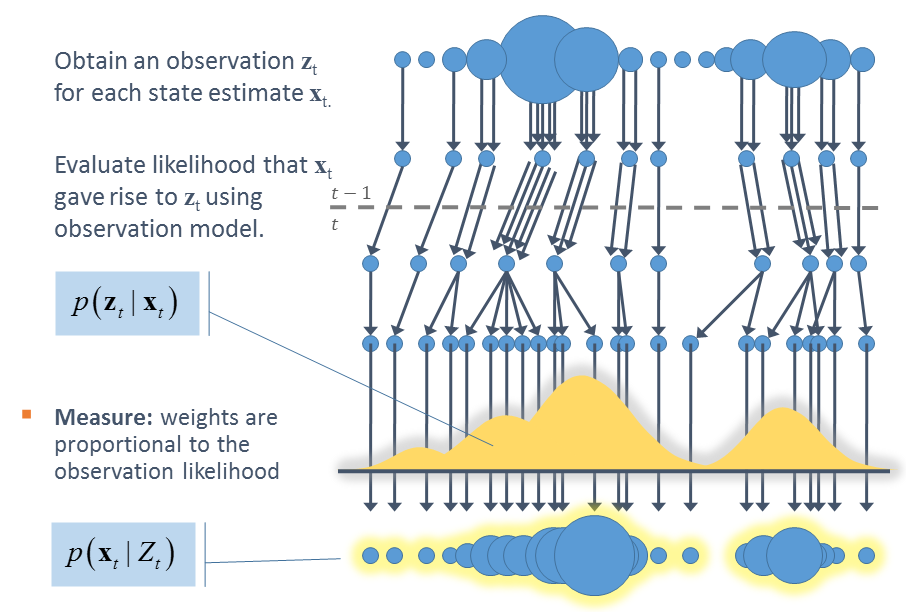
\includegraphics[width=.65\textwidth]{figures/particle_filter_flowchart.png}
    \caption{Sharath Srinivasan, towardsdatascience.com}
\end{figure}
\vfill
\end{frame}

%%%%%%%%%%%%%%%%%%%%%%%%%%%%%%%%%%%%%%%%%%%%%%%%%%%%%%%%%%%%%%%%%%%%%%%%%%%%%%%%%%%%%%%%%%%%%%%%%%%%%%%%%%%%

\begin{frame}{Reweighting}
\vfill
\begin{figure}[H]
    \centering
    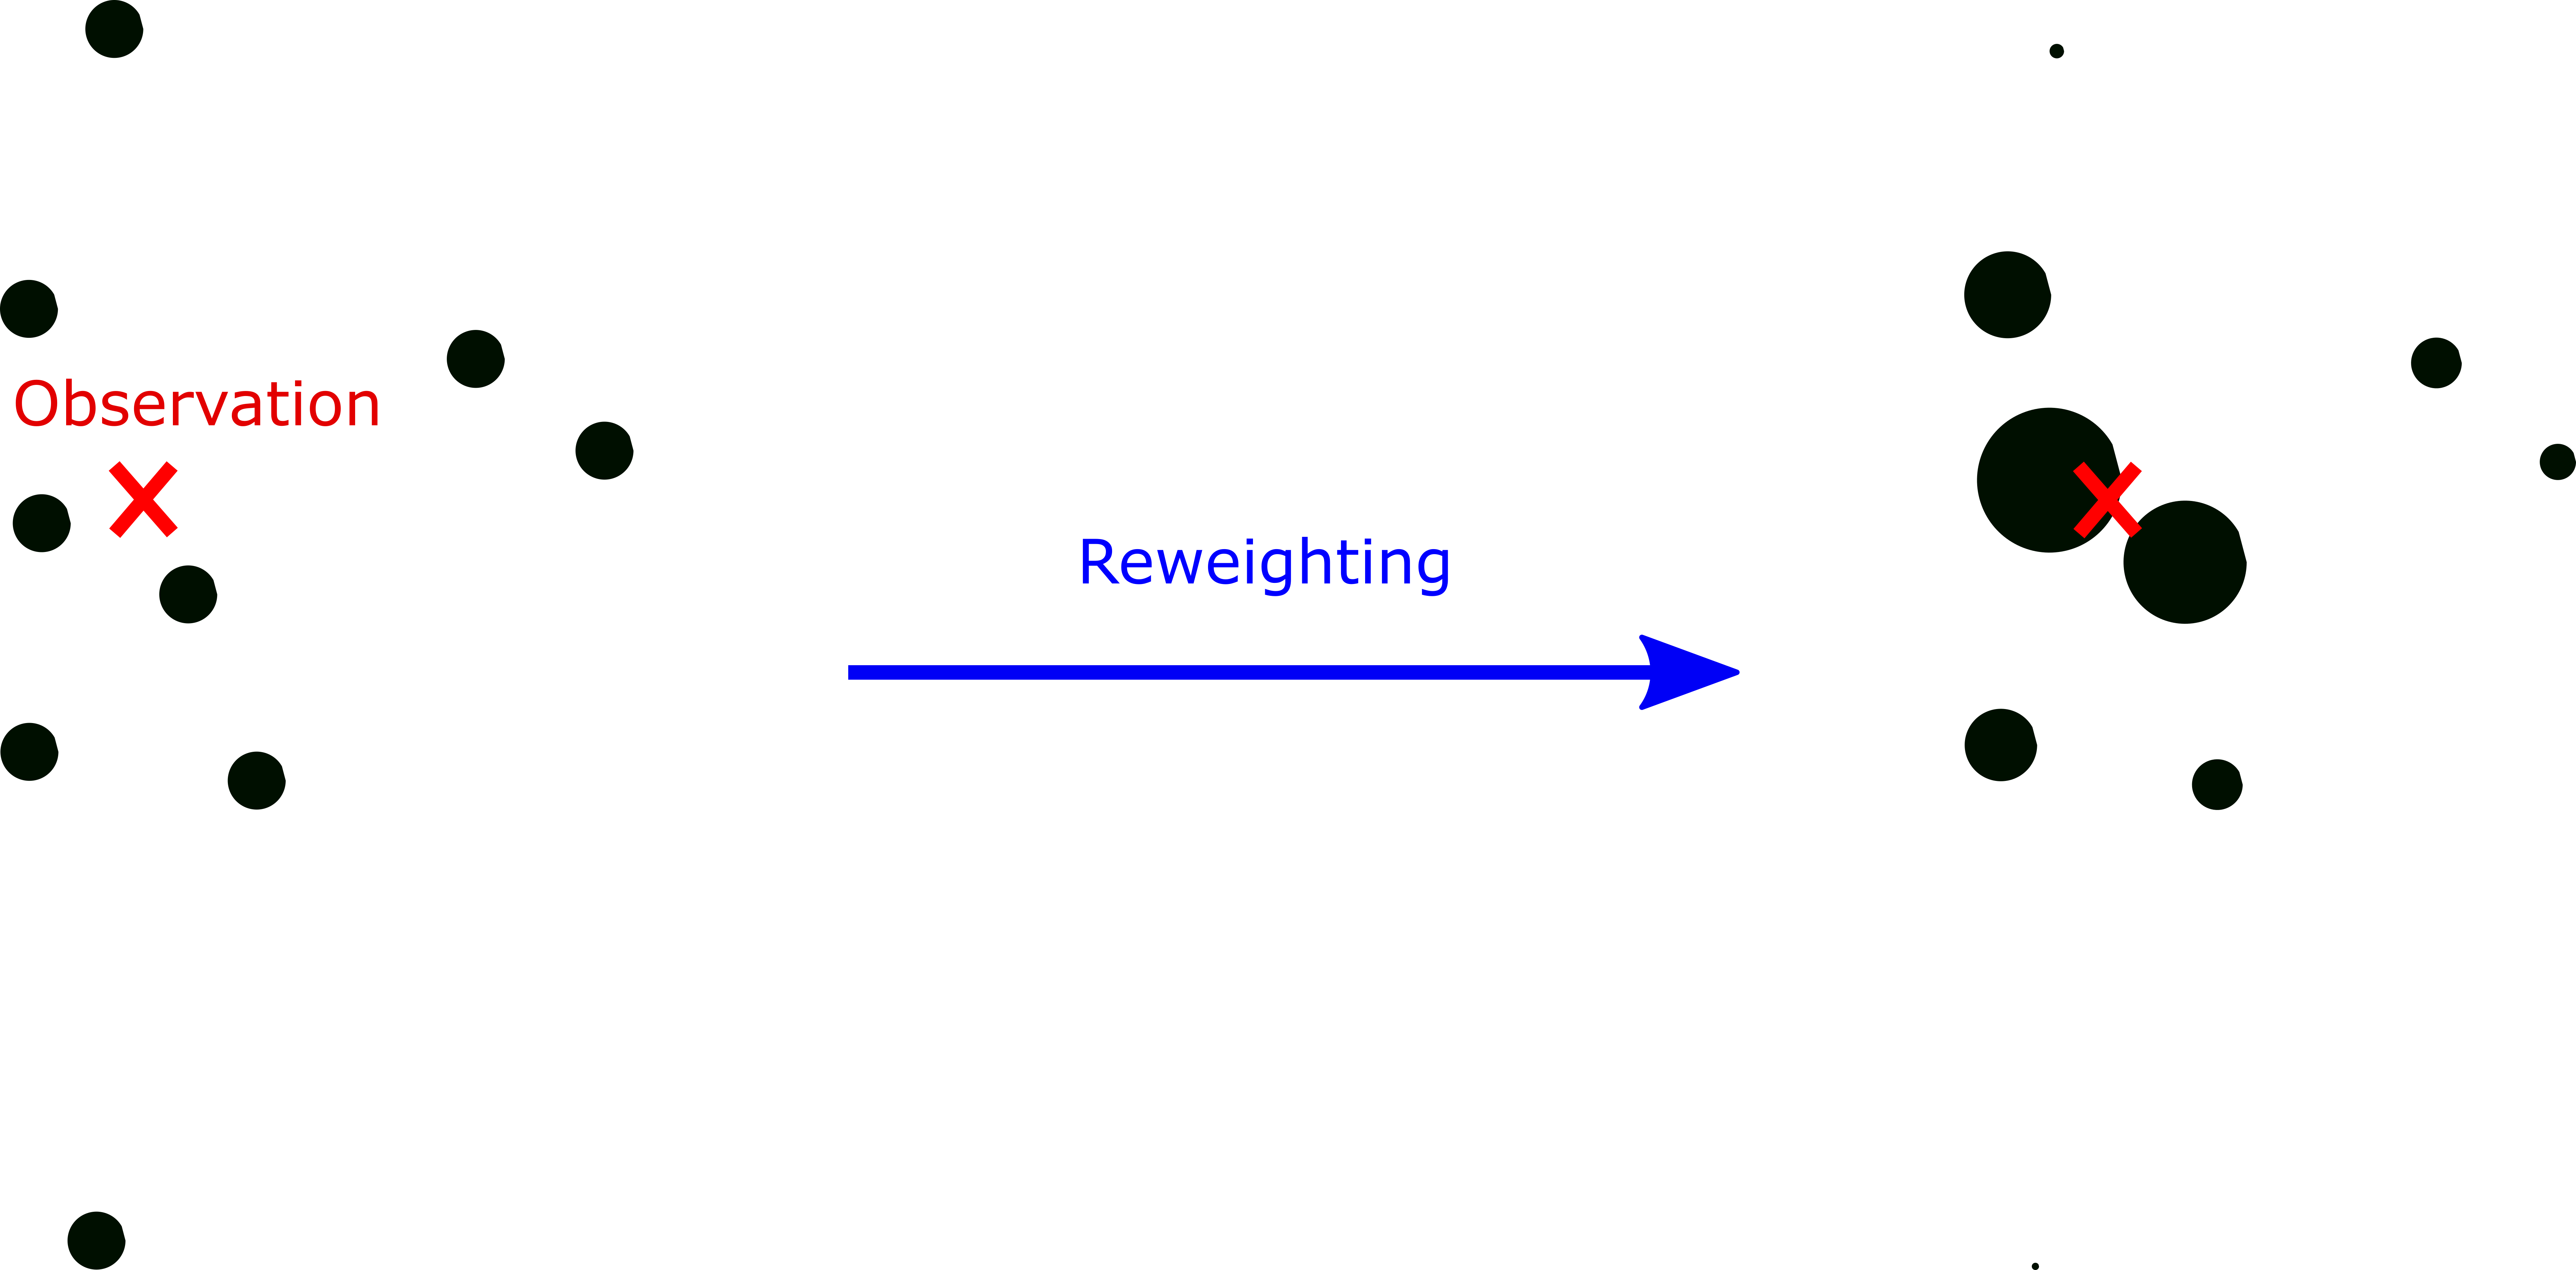
\includegraphics[width=.85\textwidth]{figures/reweighting.png}
\end{figure}
\vspace*{.25cm}
\end{frame}

%%%%%%%%%%%%%%%%%%%%%%%%%%%%%%%%%%%%%%%%%%%%%%%%%%%%%%%%%%%%%%%%%%%%%%%%%%%%%%%%%%%%%%%%%%%%%%%%%%%%%%%%%%%%

\begin{frame}{Resampling}
\vfill
\begin{itemize}
    \item At each time step, we also check the number of effective particles by $N_{\textrm{eff}} = \frac{1}{\sum_{\ell =1}^L (\weights_t^\ell)^2}$.
    \item If $N_{\textrm{eff}}$ drops below a threshold, we \boldgreen{resample} new particles with a Gaussian around the particle mean or latest observation.
\end{itemize}
\vfill
\end{frame}


%%%%%%%%%%%%%%%%%%%%%%%%%%%%%%%%%%%%%%%%%%%%%%%%%%%%%%%%%%%%%%%%%%%%%%%%%%%%%%%%%%%%%%%%%%%%%%%%%%%%%%%%%%%%

\begin{frame}{Discussion}
\vfill
    \textbf{\underline{Why PF?}} 
    \begin{itemize}
        \item PF is effective for nonlinear problems.
        \item PF captures non-Gaussian posteriors.
    \end{itemize}

\hl{Other filtering methods can't accomplish both of these.}
\vspace*{.25cm}
    \textbf{\underline{Why NOT PF?}}
    \begin{itemize}
        \item Weight degeneration in high dimensional applications.
        \item Need $L\propto \exp(MD)$ particles to avoid weight degeneration.
    \end{itemize}
\vfill
\end{frame}

%%%%%%%%%%%%%%%%%%%%%%%%%%%%%%%%%%%%%%%%%%%%%%%%%%%%%%%%%%%%%%%%%%%%%%%%%%%%%%%%%%%%%%%%%%%%%%%%%%%%%%%%%%%%

\begin{frame}{Dimension reduction}
    \textbf{\underline{Mitigating the curse of high dimensionality:}}
    \begin{itemize}
        \item Determine \boldgreen{dynamically significant} basis elements. 
        \item These are basis elements capture large scale flow patterns and coherent structures over time.
        \item Project our problem onto these basis elements to reduce the dimensionality.
    \end{itemize}
\end{frame}

%%%%%%%%%%%%%%%%%%%%%%%%%%%%%%%%%%%%%%%%%%%%%%%%%%%%%%%%%%%%%%%%%%%%%%%%%%%%%%%%%%%%%%%%%%%%%%%%%%%%%%%%%%%%

\begin{frame}{Reduction methods}
    \begin{itemize}
        \item Assimilation in the Unstable Subspace (AUS) 
        \begin{itemize}
            \item Time dependent basis elements.
            \item More computationally challenging.
        \end{itemize}
        \item Proper Orthogonal Decomposition (POD) 
        \begin{itemize}
            \item Simple and cheap to implement.
        \end{itemize}
        \item Dynamic Mode Decomposition (DMD) 
        \begin{itemize}
            \item More flexibility in choosing dynamically significant elements than POD.
            \item Needs more knowledge of the dynamics we are capturing.
        \end{itemize}
    \end{itemize}
\end{frame}

%%%%%%%%%%%%%%%%%%%%%%%%%%%%%%%%%%%%%%%%%%%%%%%%%%%%%%%%%%%%%%%%%%%%%%%%%%%%%%%%%%%%%%%%%%%%%%%%%%%%%%%%%%%%

\begin{frame}{Intuition}
    \begin{enumerate}[1.]
        \item Run the model and make observations up to time $T$.
        \item Build snapshot matrix $\snapshot = \begin{pmatrix} \vert & \vert & \cdots & \vert \\ \state_1 & \state_2 & \cdots & \state_T \\ \vert & \vert & \cdots & \vert\end{pmatrix}$.
        \item Compute the singular value decomposition $\snapshot = \boldsymbol{U \Sigma V}^\dagger$.
        \item Choose the modes corresponding to the largest $q$ singular values.
    \end{enumerate}
\end{frame}

%%%%%%%%%%%%%%%%%%%%%%%%%%%%%%%%%%%%%%%%%%%%%%%%%%%%%%%%%%%%%%%%%%%%%%%%%%%%%%%%%%%%%%%%%%%%%%%%%%%%%%%%%%%%

\begin{frame}{Projected data assimilation}
    \begin{itemize}
        \item We can now determine $M^q<M$ and $D^q<M$ significant modes for the model and data respectively.
        \item We now perform DA on the dimensionally reduced problem by working solely with the coefficients of the dominant modes.
        \item We must balance keeping enough modes to represent the dynamics, but dropping enough to have effective PF.
    \end{itemize}
\end{frame}

%%%%%%%%%%%%%%%%%%%%%%%%%%%%%%%%%%%%%%%%%%%%%%%%%%%%%%%%%%%%%%%%%%%%%%%%%%%%%%%%%%%%%%%%%%%%%%%%%%%%%%%%%%%%

\begin{frame}{Projection choices}
\vfill
    \begin{figure}[H]
        \centering
        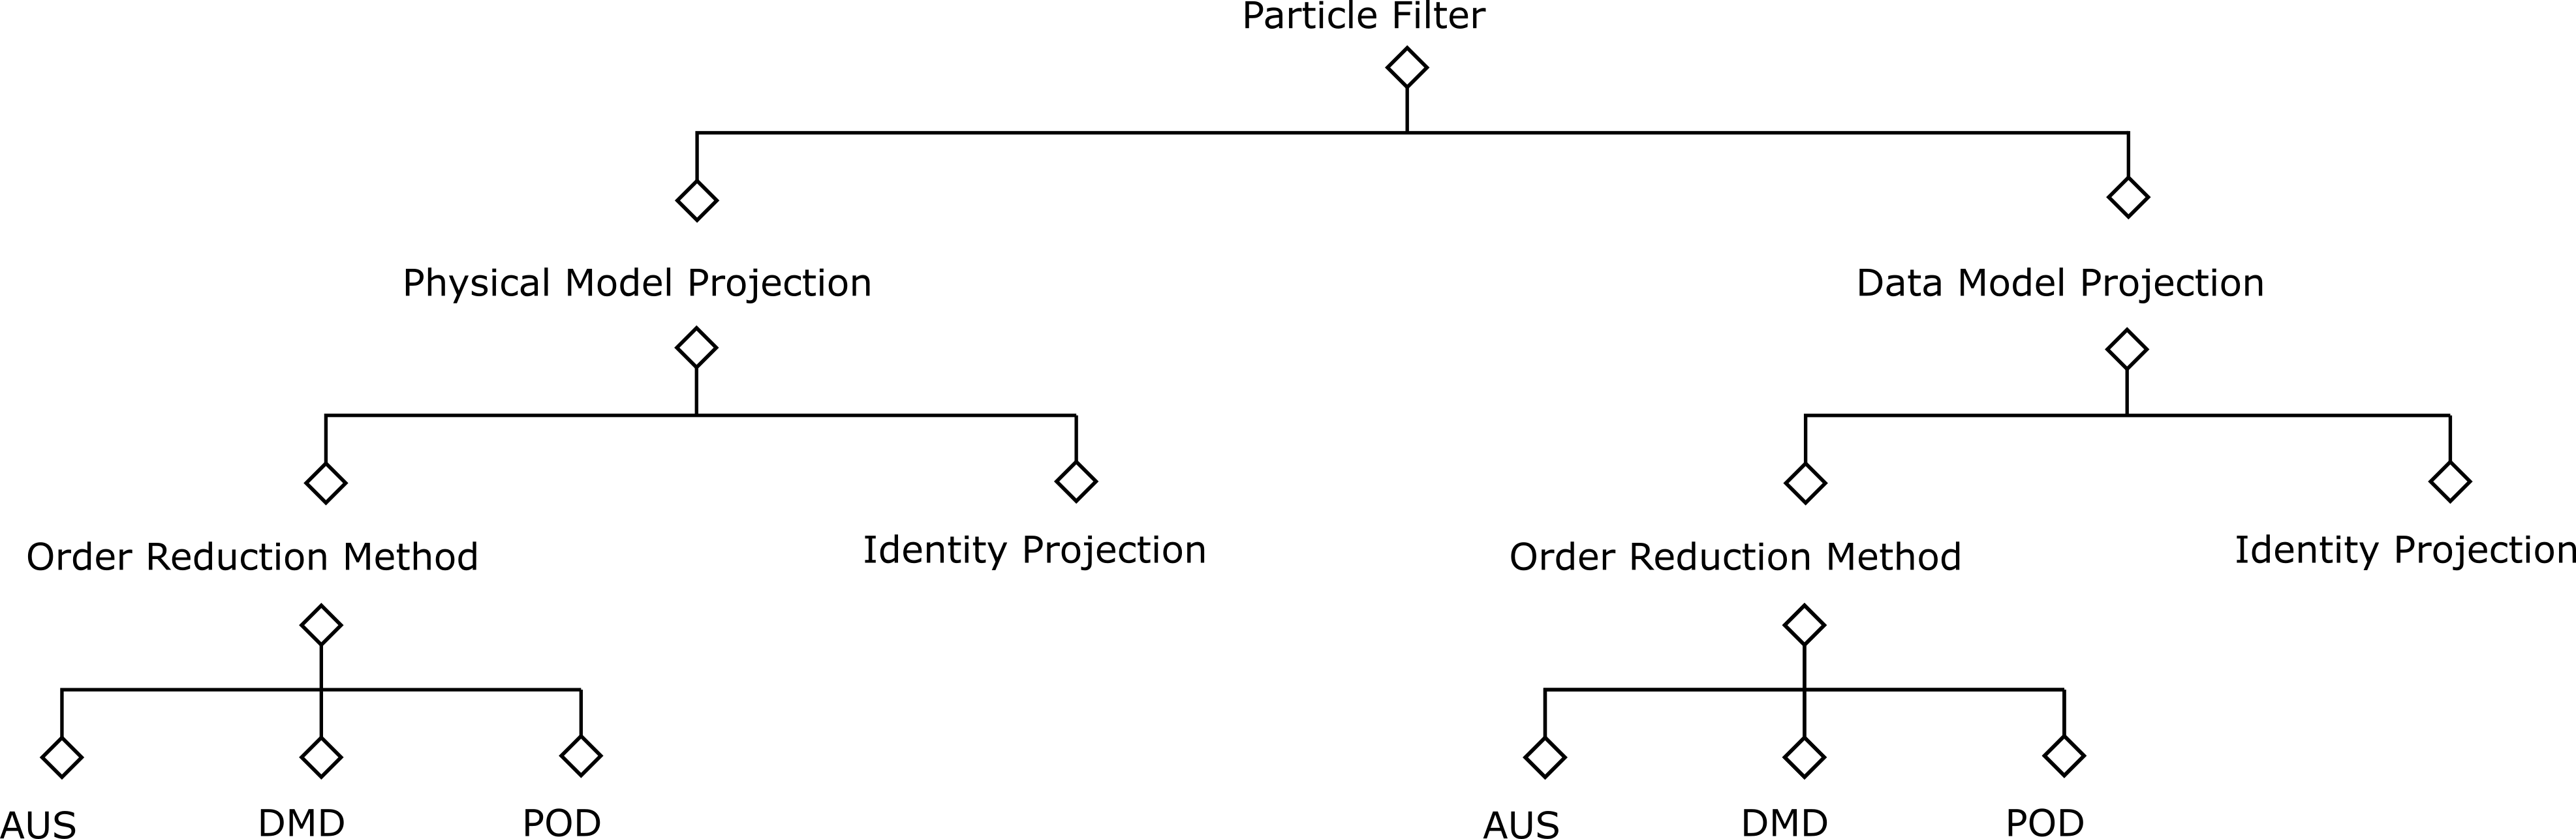
\includegraphics[width=.7\textwidth]{figures/decision_tree.png}
    \end{figure}
\vfill
\end{frame}

%%%%%%%%%%%%%%%%%%%%%%%%%%%%%%%%%%%%%%%%%%%%%%%%%%%%%%%%%%%%%%%%%%%%%%%%%%%%%%%%%%%%%%%%%%%%%%%%%%%%%%%%%%%%

\begin{frame}{What we're looking for}
\vfill
    \begin{itemize}
        \item Capture coherent structures.
        \item Low Root Mean Square Error (RMSE) from particle mean to truth.
        \item Low resampling rate.
    \end{itemize}
\vfill
\end{frame}

%%%%%%%%%%%%%%%%%%%%%%%%%%%%%%%%%%%%%%%%%%%%%%%%%%%%%%%%%%%%%%%%%%%%%%%%%%%%%%%%%%%%%%%%%%%%%%%%%%%%%%%%%%%%

\begin{frame}{RMSE}
\vfill
Our method of measuring error is the RMSE
\[
\textrm{RMSE} = \frac{(\state_t^{\textrm{truth}}-\mu_t)^\dagger \cdot (\state_t^{\textrm{truth}}-\mu_t)}{M}
\]
\vfill
\end{frame}



%%%%%%%%%%%%%%%%%%%%%%%%%%%%%%%%%%%%%%%%%%%%%%%%%%%%%%%%%%%%%%%%%%%%%%%%%%%%%%%%%%%%%%%%%%%%%%%%%%%%%%%%%%%%

\begin{frame}{Lorenz 96}
\begin{itemize}
    \item ODE describing meteorological quantities along lines of latitude.
    \item A staple comparison for other assimilation schemes.
    \item We ran with $M=100$ and $F=3.5$. Truth below. 
\end{itemize}
\begin{figure}[H]
    \centering
    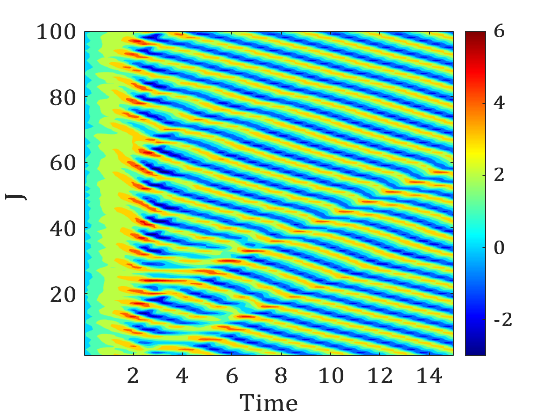
\includegraphics[width=.5\textwidth]{figures/L96_F3.5N100.png}
\end{figure}
\end{frame}

\begin{frame}{Results}
\begin{columns}
    \begin{column}{.49\textwidth}
\begin{figure}[H]
\centering
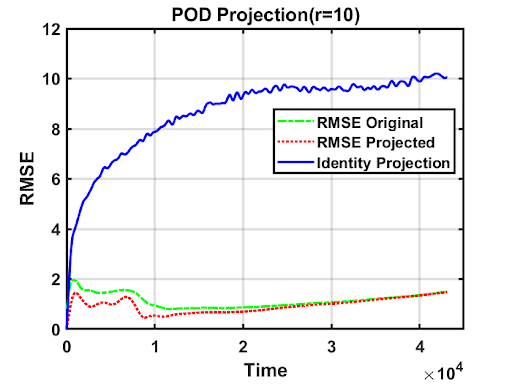
\includegraphics[width=\textwidth]{figures/l96_pod10.png}
\caption{POD reduction to $M^q=10$.}
\end{figure}
    \end{column}

 \begin{column}{.49\textwidth}
\begin{figure}[H]
\centering
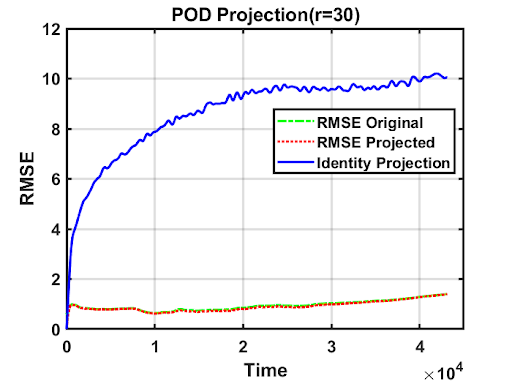
\includegraphics[width=\textwidth]{figures/l96_pod30.png}
\caption{POD reduction to $M^q=30$.}
\end{figure}
 \end{column}
\end{columns}
\end{frame}



%%%%%%%%%%%%%%%%%%%%%%%%%%%%%%%%%%%%%%%%%%%%%%%%%%%%%%%%%%%%%%%%%%%%%%%%%%%%%%%%%%%%%%%%%%%%%%%%%%%%%%%%%%%%

%\begin{frame}{Shallow water equations}
%    \textbf{\underline{Model of interest:}} Shallow water equations
%    \begin{align*}
%        \frac{\partial u}{\partial t} &= \left(-\frac{\partial u}{\partial y} + f\right) v - \frac{\partial}{\partial x} \left(\frac{1}{2} u^2 +gh\right) + \nu \Delta u - c_b u\\
%        \frac{\partial v}{\partial t} &= -\left(\frac{\partial v}{\partial x}+f\right) u - \frac{\partial}{\partial y} \left(\frac{1}{2} v^2 +gh\right) + \nu \Delta v - c_b v\\
%        \frac{\partial h}{\partial t} &= -\frac{\partial}{\partial x} ((h+\underline{h})u)-\frac{\partial}{\partial y} ((h+\underline{h})v).
%    \end{align*}
%
%    \begin{itemize}
%        \item $u(x,y,t)$ and $v(x,y,t)$ are velocity in the $x$ and $y$ directions respectively.
%        \item $h(x,y,t)$ is the height of the column of water at $(x,y)$ at time $t$.
%    \end{itemize}
%\end{frame}

%%%%%%%%%%%%%%%%%%%%%%%%%%%%%%%%%%%%%%%%%%%%%%%%%%%%%%%%%%%%%%%%%%%%%%%%%%%%%%%%%%%%%%%%%%%%%%%%%%%%%%%%%%%%

\begin{frame}{Shallow water equations}
    \begin{itemize}
        \item PDE to solve for the height $h(x,y,t)$ of a column of water.
        \item Discretized $x$ and $y$ to get a grid of size $38,100$ (dimension of the problem).
        \item Truth was given by barotropic instability \url{http://www.met.reading.ac.uk/~swrhgnrj/shallow_water_model/}
    \end{itemize}

For every run we have
    \begin{itemize}
        \item Total particles $L=20$.
        \item Observation time is every 60 seconds
        \item Covariances: $\modelcovariance = I$, $\observationcovariance = 0.01I$.
    \end{itemize}
\end{frame}

%%%%%%%%%%%%%%%%%%%%%%%%%%%%%%%%%%%%%%%%%%%%%%%%%%%%%%%%%%%%%%%%%%%%%%%%%%%%%%%%%%%%%%%%%%%%%%%%%%%%%%%%%%%%

\begin{frame}{Qualitative results}
    \begin{columns}
    \begin{column}{.49\textwidth}
\begin{figure}[H]
\centering
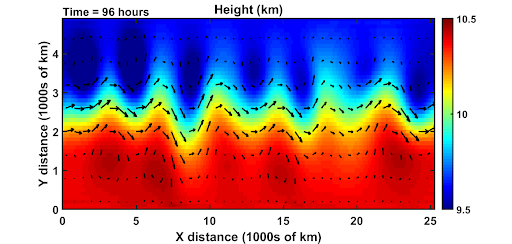
\includegraphics[width=\textwidth]{figures/swe_truth.png}
\caption{Truth run for shallow water equations.}
\end{figure}
    \end{column}

 \begin{column}{.49\textwidth}
\begin{figure}[H]
\centering
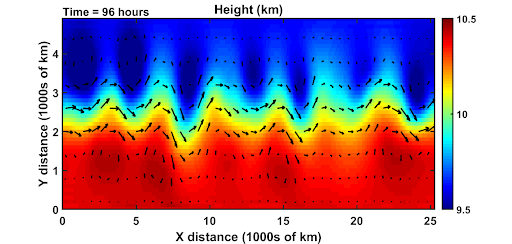
\includegraphics[width=\textwidth]{figures/swe_pod10.png}
\caption{POD projection with $M^q=D^q=100$ run for shallow water equations.}
\end{figure}
 \end{column}
\end{columns}
\end{frame}

%%%%%%%%%%%%%%%%%%%%%%%%%%%%%%%%%%%%%%%%%%%%%%%%%%%%%%%%%%%%%%%%%%%%%%%%%%%%%%%%%%%%%%%%%%%%%%%%%%%%%%%%%%%%

\begin{frame}{Results}
    \begin{figure}[H]
        \centering
        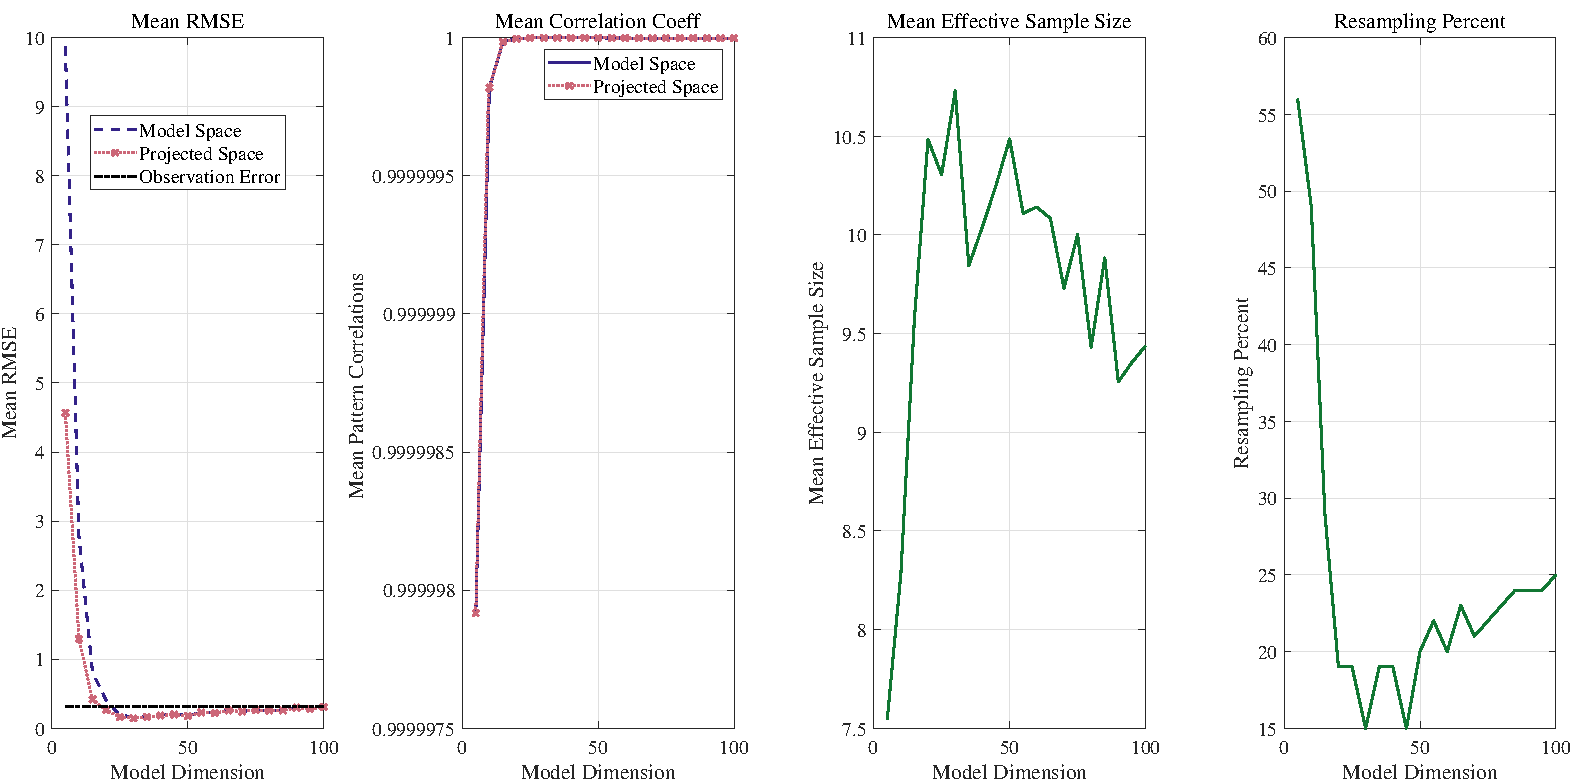
\includegraphics[width=\textwidth]{figures/SWE_physical_proj_DMD_inth1000.png}
        \caption{Fixed $D^q = 10$ and varied $M^q$.  Observed every 1000th gridpoint every 60 seconds.}
    \end{figure}
\end{frame}

%%%%%%%%%%%%%%%%%%%%%%%%%%%%%%%%%%%%%%%%%%%%%%%%%%%%%%%%%%%%%%%%%%%%%%%%%%%%%%%%%%%%%%%%%%%%%%%%%%%%%%%%%%%%

\begin{frame}{Collaborators}
    \begin{itemize}
        \item Aishah Albarakati, Clarkson University, U.S.;
        \item Rose Crocker, The University of Adelaide, Australia;
        \item Juniper Glass-Klaiber, Mount Holyoke College, U.S.;
        \item Sarah Iams, Harvard University, U.S.;
        \item Noah Marshall, University of British Colombia, Canada;
        \item Erik Van Vleck, University of Kansas, U.S.
    \end{itemize}
\end{frame}

\begin{frame}{Support and funding}
\begin{figure}
     \centering
     \begin{subfigure}[b]{0.3\textwidth}
         \centering
         
\includegraphics[width=\textwidth]{figures/mcrn.png}
     \end{subfigure}
     \hfill
     \begin{subfigure}[b]{0.35\textwidth}
         \centering
         
\includegraphics[width=\textwidth]{figures/aim.jpg}
     \end{subfigure}
     \hfill
     \begin{subfigure}[b]{0.3\textwidth}
         \centering
         
\includegraphics[width=\textwidth]{figures/nsf.png}
     \end{subfigure}
\end{figure}
\end{frame}

\end{document}

